% Modelo de slides para projetos de disciplinas do Abel
\documentclass[aspectratio=169,11pt]{beamer}

\usetheme[%
 sectionpage=none,%
 subsectionpage=progressbar%
 ]{metropolis}
\setbeamercovered{transparent}
\useoutertheme{infolines}
\setbeamersize{text margin left=1cm,text margin right=1cm}
\setbeamertemplate{part page}
{
  \begin{centering}
    \begin{beamercolorbox}[sep=16pt,center]{part title}
      \usebeamerfont{part title}\insertromanpartnumber.~\insertpart\par
    \end{beamercolorbox}
  \end{centering}
}

\usepackage[czech]{babel}
\usepackage{graphicx}
\usepackage{enumitem}
\usepackage{amsmath}
\usepackage{mathtools}
\usepackage{tcolorbox}

\tcbset{%
 sharp corners=all,%
 boxsep=7pt,%
 fonttitle=\bfseries,%
 colback=gray!30!white,%
 colframe=mDarkTeal,%
 boxrule=1pt%
}

\title{PSEUDOKÓD}
\date{\today}
\author{Adam Klepáč}
\institute[GEVO]{Gymnázium Evolution Jižní Město}

% enumerate global settings
\setlist[enumerate,1]{label=\arabic*.}
\setlist[enumerate,2]{label=\alph*)}
\setlist[itemize,1]{label=\textbullet}

\begin{document}

\maketitle

\part[Předmluva]{Předmluva}

\begin{frame}
 \partpage
\end{frame}

\begin{frame}
 \frametitle{Obsah}
 \tableofcontents
\end{frame}

\section[Program]{Program}
\subsection[CPU]{CPU}

\begin{frame}
 \frametitle{Co je CPU?}
 \begin{columns}
  \begin{column}{.3\textwidth}
   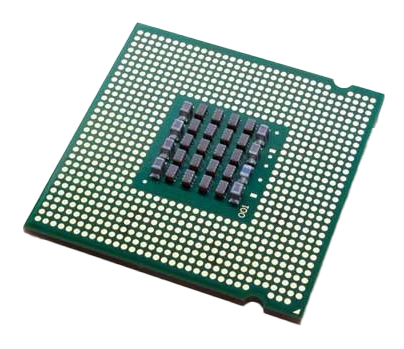
\includegraphics[width=\textwidth]{cpu}
  \end{column}
  \begin{column}{.7\textwidth}
   \begin{tcolorbox}
    CPU (\textbf{C}entral \textbf{P}rocessing \textbf{U}nit) je elektrický
    obvod, který vykonává \alert{instrukce} tvořící \alert{počítačový program}.
   \end{tcolorbox}
  \end{column}
 \end{columns}
\end{frame}

\subsection[Operace]{Operace}

\begin{frame}
 \frametitle{Fetch}
 \begin{tcolorbox}[title=Fetch,center,width=.95\textwidth]
  CPU \alert{vyzvedne} instrukci z programu.
 \end{tcolorbox}
 \begin{itemize}
  \item Instrukce je v programu uložena jako posloupnost nul a jedniček.
  \item Poloha (adresa) instrukce je dána čítačem (program counter). Postaru se
   mu někdy říká `hlava'.
  \item Čítač uchovává adresu poslední instrukce a po přečtení se posune o délku
   (v~bitech) zpracovávané instrukce.
 \end{itemize}
\end{frame}

\begin{frame}
 \frametitle{Decode}
 \begin{tcolorbox}[title=Decode,center,width=.95\textwidth]
  CPU \alert{přeloží} načtenou instrukci.
 \end{tcolorbox}
 \begin{itemize}
  \item Prvních pár bitů v instrukci obvykle značí operaci, která se má provést.
  \item Zbývající bity jsou pak například adresy operandů v paměti.
 \end{itemize}
\end{frame}

\begin{frame}
 \frametitle{Execute}
 \begin{tcolorbox}[title=Execute,center,width=.95\textwidth]
  CPU \alert{provede} přeloženou instrukci.
 \end{tcolorbox}
 \begin{itemize}
  \item V závislosti na architektuře CPU, instrukce obsahují buď jedinou akci
   nebo posloupnost akcí.
  \item Výsledek je uložen ve vnitřní paměti CPU. Uložení do vnější paměti
   (třeba RAM nebo disk) musí být obsahem nějaké další instrukce.
 \end{itemize}
\end{frame}

\subsection[Instrukce]{Typy instrukcí}

\begin{frame}
 \centering\Huge Díky za pozorst.
\end{frame}

\end{document}
